\subsection*{Line-Of-Sight Propagation}
\paragraph{}
At low frequency (below approximately 3 MHz) radio signals travel as ground waves, which follow the Earth's curvature due to diffraction with the layers of the atmosphere.
However, at higher frequencies and in lower levels of the atmosphere, neither of these effects are significant. Thus any obstruction between the transmitting antenna (transmitter) and the receiving antenna (receiver) will block the signal, just like the light that the eye may sense. Therefore, since the ability to visually see a transmitting antenna (disregarding the limitations of the eye's resolution) roughly corresponds to the ability to receive a radio signal from it, the propagation characteristic of VHF and higher radio frequency (>30 MHz) paths is called line-of-sight. The farthest possible point of propagation is referred to as the radio horizon.

The radio horizon is the locus of points at which direct rays from an antenna are tangential to the surface of the Earth. If the Earth were a perfect sphere and there were no atmosphere, the radio horizon would be a circle.

This way the greatest distance at which a receiver can see the transmiter is explained in the following figure:

%\begin{figure}[hb]
%  	\centering
% 	
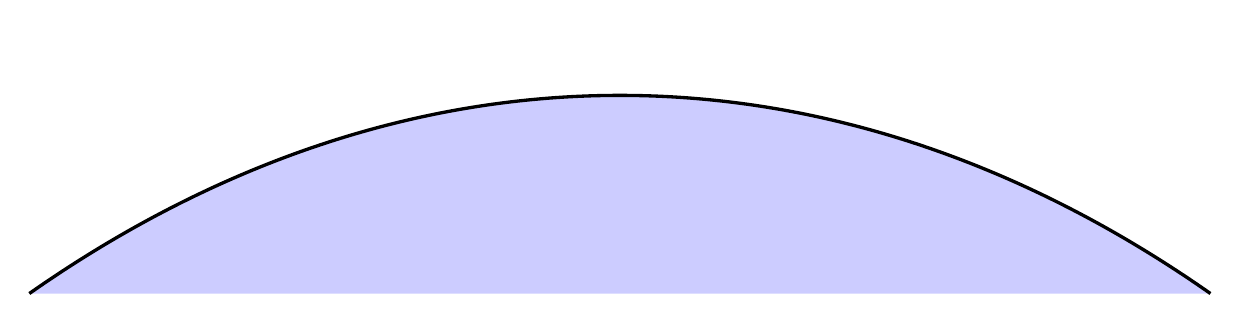
\begin{tikzpicture}
\draw[very thick, draw=black, fill=blue, fill opacity=0.2] (0,0) to [out=35,in=145] (15,0);
\end{tikzpicture}
%  	\caption[Pipeline survey]{Scenario}
%\end{figure}
